\documentclass[12pt]{book}

\usepackage[utf8]{inputenc}
\usepackage[french]{babel}
\usepackage[T1]{fontenc}

\usepackage{tikz}
\usetikzlibrary{patterns}
\usepackage{graphicx}
\usepackage{caption}
\usepackage{svg}
\usepackage{csquotes}
\usepackage{esdiff}
\usepackage{amsmath}
\usepackage{amsthm}
\usepackage{mathrsfs}
\usepackage{siunitx}
\usepackage{amsthm}

\newcounter{myremark}[chapter]
\renewcommand{\themyremark}{Remarque \thechapter.\arabic{myremark}}
\makeatletter
\newenvironment{remark}[1][]{
    \refstepcounter{myremark}
    \noindent\ignorespaces
    \begin{description}
        \item[\themyremark\space\ifx\relax#1\relax\else(#1) \fi:]
            }{
    \end{description}%
}
\makeatother


\newtheoremstyle{bfnote}
{}{}
{\itshape}{}
{\bfseries}{.}
{ }{\thmname{#1}\thmnumber{ #2}\thmnote{ (#3)}}
\theoremstyle{bfnote}

\theoremstyle{bfnote}
\newtheorem{problem}{Problem}[chapter]

\usepackage[a4paper, margin = 1in]{geometry}


\DeclareSIUnit{\RPM}{RPM}

\begin{document}

\chapter{Formulation du Problème} % (fold)
\label{chap:Formulation_du_Probleme}
Nous allons calculer le champ d'écoulement de l'air à l'intérieur de l'entrée du moteur. À cette fin, une simulation complète du domaine à l'aide des équations de Navier-Stokes représente l'approche la plus rigoureuse. Cependant, résoudre l'intégralité des équations de Navier-Stokes sans approximation semble coûter cher en termes de calcul, d'autant plus que le problème ne présente aucun effet instable. Nous justifierons ce fait plus tard. Cependant, nous proposons un prototype géométrique pour le champ d'écoulement, défini comme suit:

\begin{problem}
    Considérons un cylindre de rayon $R_2$ et de longueur $H_2$. À l'intérieur du cylindre, se trouve un cône de rayon $R_1$ et de hauteur $H_1$ (demi-angle $\psi$). Ce cône est situé à l'extrémité du cylindre. L'écoulement à travers le cylindre a une vitesse non perturbée $U_{\infty}$ au début de l'entrée. Le cône tourne à une vitesse angulaire $\omega$, ce qui induit une composante tourbillonnaire dans le champ d'écoulement.
\end{problem}

Dans les conditions de croisière, l'air possède les propriétés suivantes:
\[
\begin{array}{lcl}
    h & \cdots\cdots\cdots & \SI{10000}{\meter} \\
    \rho_\infty & \cdots\cdots\cdots & \SI{0.38671}{\kilogram\per\meter^3} \\
    T_\infty & \cdots\cdots\cdots & \SI{238.15}{\kelvin} \\
    p_\infty & \cdots\cdots\cdots & \SI{26436}{\pascal} \\
    c & \cdots\cdots\cdots & \SI{309.36}{\meter\per\second} \\
    \mu & \cdots\cdots\cdots & \SI{0.00001552}{\pascal\cdot\second} \\
\end{array}
\]
Ces valeurs sont calculées en utilisant les conditions de l'ISA avec le température au niveau de la mer de $T = \SI{15}{\degreeCelsius}$.

Dans les conditions de croisière, nous ne prenons pas en compte les effets des vortex au sol. Tous les effets secondaires, tels que les vibrations de l'entrée de nacelle et du cône, ainsi que la rugosité des surfaces, seront négligés. De plus, comme le nombre de Mach de l'écoulement libre est d'environ $0.85$, correspondant à la vitesse de croisière de l'avion, il n'y a pas de raison d'ignorer a priori la compressibilité de l'écoulement. Cependant, nous la négligerons, car le profil de l'écoulement à l'entrée ne varie pas de manière significative en termes de température, de pression et de densité. À une première approximation, nous considérons que le champ d'écoulement est incompressible.

On estime maintenant qualitativement l'effet de la viscosité sur le premier écoulement. Pour ce faire, le nombre de Reynolds autour du cône est calculé:
\begin{align}
    \mathrm{Re} \approx \dfrac{\rho_{\infty} \Omega R_1}{\mu_{\infty}} = \dfrac{\SI{0.38671}{\kilogram\per\meter^3} \times \SI{319}{\radian\per\second} \times \SI{0.25}{\meter}}{\SI{0.00001552}{\pascal\cdot\second}} \approx 2 \times 10^6.
\end{align}
Ce calcul découle des faits suivants:
\begin{enumerate}
    \item Le cône (spinner) est directement lié à l'arbre basse pression (LP), qui fonctionne dans une plage de vitesse d'environ $\SI{3000}{\RPM}$ à $\SI{5000}{\RPM}$ en vitesse de croisière.
    \begin{align*}
        \Omega \approx \dfrac{\SI{4000}{\RPM} \times 2 \pi}{\SI{60}{\second\per\minute}} \approx \SI{420}{\radian\per\second}.
    \end{align*}
    \item Le rayon de la base du cône correspond au rayon du moyeu du ventilateur, dicté par le ratio moyeu/voilure. Pour un moteur turbofan moderne typique, ce ratio varie de $0.2$ à $0.35$. Pour un moteur turbofan avec un diamètre de ventilateur de $\SI{2}{\meter}$, on a:
    \begin{align*}
        R_1 \approx 0.25 \times \SI{1}{\meter} = \SI{0.25}{\meter}.
    \end{align*}
\end{enumerate}

Ce nombre de Reynolds est très élevé, ce qui nous force à calculer le champ d'écoulement en utilisant le modèle de « très grand nombre de Reynolds ». En effet, le champ d'écoulement est divisé en deux régions: la région principale, où les effets visqueux sont négligeables, et la région de la couche limite, où tous les effets visqueux significatifs sont concentrés. Dans la couche limite, nous calculerons tous les effets dus à la viscosité en utilisant des perturbations à partir de la solution non visqueuse. La même conclusion peut être tirée pour l'écoulement près de la paroi de l'entrée moteur (nacelle). En fait, le nombre de Reynolds au niveau de la paroi est:
\begin{align*}
    \mathrm{Re} \approx \dfrac{\rho_\infty U_{\text{paroi}} R_2}{\mu_\infty} = \dfrac{\SI{0.38671}{\kilogram\per\meter^3} \times \SI{250.75}{\meter\per\second} \times \SI{0.5}{\meter}}{\SI{0.00001552}{\pascal\cdot\second}} \approx 3 \times 10^6.
\end{align*}
Ce calcul provient du fait que l'écoulement à la condition de croisière a une vitesse $U_{\text{paroi}} \approx \SI{250.75}{\meter\per\second}$ pour Mach $0.85$, et que le rayon de l'entrée moteur est approximé à environ $\SI{0.5}{\meter}$.

En suivant le modèle de « très grand nombre de Reynolds », nous poursuivons comme suit:
\begin{enumerate}
    \item Supposons que l'écoulement est non visqueux et trouvons une solution non visqueuse pour l'ensemble du champ d'écoulement.
    \item Considérons la couche limite comme une petite perturbation de la solution non visqueuse et essayons de la résoudre pour obtenir le profil de pression et de frottement le long de la surface du cône.
\end{enumerate}

Le premier sous-problème est important pour l'intégration de l'équation du mouvement des débris de glace détachés, et le second est crucial pour notre analyse du processus de détachement lui-même.
% chapter Formulation du Problème (end)

\section{Solution Non-Visqueuse} % (fold)
\label{sec:Solution_Non_Visqueuse}
Bien que le cône ait une vitesse de rotation non nulle $\Omega$, le champ d'écoulement est entièrement potentiel, car l'écoulement est non-visqueux et ne peut donc induire aucune rotation à partir du cône. Cela implique que le champ d'écoulement est potentiel:
\begin{align}
    \Delta \phi(x, y, z) = 0.
\end{align}
En raison de l'axisymétrie du domaine, nous pouvons utiliser les coordonnées cylindriques $r, \theta, z$, où $z$ est l'axe du cylindre orienté de l'entrée à la sortie. Si la direction de la vitesse d'entrée $\underline{U}_\infty = U_\infty \underline{e}_z$ reste constante avec $U_\infty$ constant, alors la variable $\theta$ n'intervient pas dans le problème, et on peut écrire:
\begin{align}
    \Delta \phi(r, z) = 0.
\end{align}

La condition limite pour cet écoulement potentiel est que les vitesses normales à la surface du cône et au mur doivent être nulles:
\begin{align}
    & \diffp{\phi}{r}(r = R_2) = 0\\
    & {\nabla \phi} \cdot \underline{n}_{\text{cône}} = 0.
\end{align}
À l'entrée de l'inlet, la vitesse doit être uniforme:
\begin{align}
    \dfrac{1}{r} \diffp{\phi}{r}(z = H_1 - H_2) & = U_\infty \\
    - \dfrac{1}{r} \diffp{\phi}{z}(z = H_1 - H_2) & = 0
\end{align}
Cette hypothèse repose sur le fait qu'un écoulement uniforme n'interfère pas avec les performances du moteur. Nous reviendrons plus tard sur le problème de la non-uniformité.

À la sortie de l'inlet, nous pouvons supposer que l'écoulement est uniforme, car le cône, conçu pour des raisons d'ingénierie, est utilisé pour corriger l'écoulement d'air et garantir l'uniformité de l'écoulement d'entrée avant qu'il n'entre dans le ventilateur ou le compresseur. Cela vise encore à assurer les performances souhaitées du moteur. Par conséquent, nous pouvons écrire:
\begin{align}
    & \diffp{\phi}{z}(z = H_1) = U_2 \\
    & \diffp{\phi}{r}(z = H_1) = 0
\end{align}
Mais cette hypothèse n'est pas physiquement réaliste, car elle correspondrait à une déviation de l'écoulement plutôt qu'à son rôle de correction. Ainsi, nous prolongeons le mur de l'inlet d'une longueur $H_3$ et ajoutons une base cylindrique au cône d'une hauteur $H_3$ pour canaliser l'écoulement. Ce domaine imaginaire ne contribue pas à la solution finale mais aide à simuler l'écoulement de manière plus naturelle. Nous extrayons donc uniquement le domaine physique. Il n'y a pas de contrainte stricte sur la dimension $H_3$, mais nous mènerons plusieurs études de cas pour trouver la valeur optimale de $H_3$, afin que la solution ne soit pas trop coûteuse en termes de calcul tout en conservant la précision. Nous représentons le nouveau domaine comme suit:
\begin{figure}[h!]
    \centering
    \begin{tikzpicture}
        \draw[fill=blue!20, draw=black, thick] (0,0) -- (3,0) -- (6,2) -- (9,2) -- (9,4) -- (0,4) -- (0,0) -- cycle;
        \draw[dashed] (3,0) -- (9,0) ;
        \draw[dashed] (9,0) -- (9,2) ;
        \draw[dashed] (6,2) -- (6,4) ;
        \fill[pattern=north east lines] (6,2) rectangle (9,4);
        \node[below] at (4.5,1) {$\mathscr{B}_1$};
        \node[below] at (9.5,3) {$\mathscr{B}_2$};
        \node[below] at (-0.5,2) {$\mathscr{B}_3$};
        \node[below] at (4.5,4.8) {$\mathscr{B}_4$};
        \node[below] at (6.75,1) {spinner};
    \end{tikzpicture}
    \caption{Modèle de l'inlet moteur avec la région hachurée représentant le domaine imaginaire. La figure ne montre que la face coupée $\theta = 0$ en raison de l'axisymétrie.}
    \label{fig:simplified_flow_dom}
\end{figure}

\subsection{Équation de Laplace avec Condition de Dirichlet pour la Fonction de Courant} % (fold)
\label{subsec:Equation_de_Laplace_avec_Condition_de_Dirichlet_pour_la_Fonction_de_Courant}

Comme discuté précédemment, la solution non-visqueuse est formulée à partir de la fonction de courant. La fonction de courant est constante le long de chaque ligne de courant, ce qui nous permet de résoudre le problème à l'aide de l'équation de Laplace avec condition de Dirichlet:
\begin{align}
    \Delta \psi(r, z) = 0,
\end{align}
où les vitesses sont calculées comme suit:
\begin{align}
    u_z = \dfrac{1}{r} \diffp{\phi}{r}(r,z) \quad \text{et} \quad u_r = - \dfrac{1}{r} \diffp{\phi}{r}(r, z).
\end{align}

Nous représentons le domaine d'écoulement par la figure suivante (Fig.~\ref{fig:simplified_flow_dom}) où nous ajoutons un domaine imaginaire pour structurer l'écoulement:
\begin{enumerate}
    \item Le bord $\mathscr{B}_1$ représente l'axe $z$ de $z = H_1 - H_2$ au sommet du cône $z = 0$, ainsi que la surface du spinner et la surface $r = R_1$ de $z = H_1$ à $H_3$. $\mathscr{B}_1$ est une ligne de courant.
    \item Le bord $\mathscr{B}_2$ représente la sortie de l'inlet.
    \item Le bord $\mathscr{B}_3$ représente l'entrée de l'inlet moteur.
    \item Le bord $\mathscr{B}_4$ représente le mur de l'inlet.
\end{enumerate}

Avec cette convention de noms de domaine, nous pouvons directement écrire la condition limite pour la fonction de courant:
\begin{align}
    \left. \psi \right|_{\mathscr{B}_1} = 0, \quad \left. \psi \right|_{\mathscr{B}_2} = \dfrac{1}{2} U_2 \left( r^2 - R_1^2 \right), \quad \left. \psi \right|_{\mathscr{B}_3} = \dfrac{1}{2} U_1 R_1^2, \quad \left. \psi \right|_{\mathscr{B}_4} = \dfrac{1}{2} U_1 r^2
\end{align}
Les conditions sur $\mathscr{B}_1$ et $\mathscr{B}_4$ sont dues au fait que $\psi$ est constant le long de la ligne de courant. La valeur absolue de celles-ci n'est pas importante tant que leur différence $\left. \psi \right|_{\mathscr{B}_4} - \left. \psi \right|_{\mathscr{B}_1} = U_1 R_2^2/2$ représente le débit volumique. Ainsi, nous choisissons $\left. \psi \right|_{\mathscr{B}_1} = 0$ pour simplifier les calculs. La vitesse $U_2$ à la sortie est calculée par la conservation de la masse comme suit:
\begin{align}
    U_2 = U_1 \dfrac{R_1^2}{R_1^2 - R_2^2}
\end{align}
% subsection Équation de Laplace avec Condition de Dirichlet pour la Fonction de Ligne de Courant (end)

\subsection{Solution par la Méthode des Éléments Finis} % (fold)
\label{subsec:Solution_par_la_Méthode_des_Éléments_Finis}

En raison de la nature axisymétrique du champ d'écoulement, nous souhaitons appliquer l'élément axisymétrique. Ce choix permettra de réduire considérablement le coût computationnel par rapport à un modèle tridimensionnel complet. La philosophie adoptée consiste à convertir un élément annulaire tridimensionnel en un élément bidimensionnel. Pour ce faire, nous représentons la grille pour la face coupée $\theta = 0$.

\begin{figure}[h!]
    \centering
    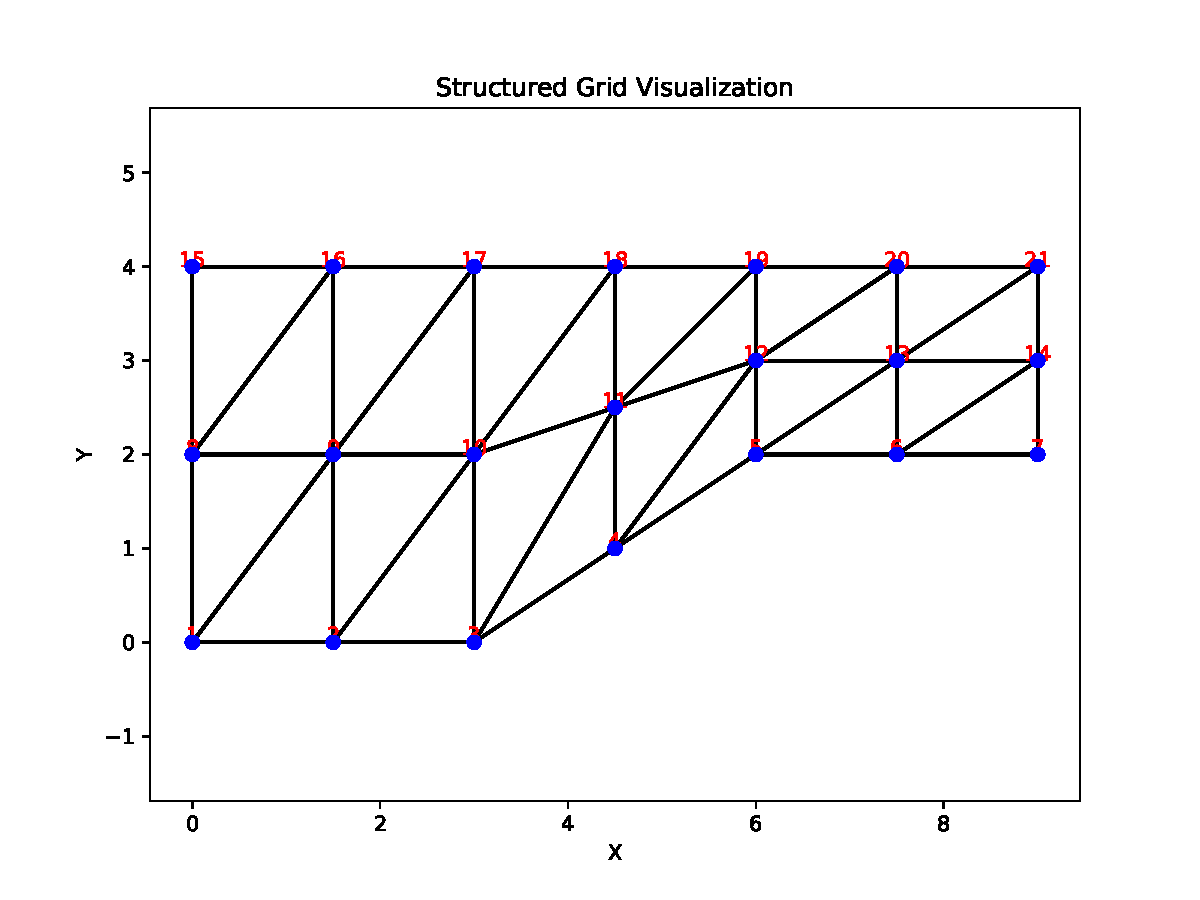
\includegraphics[width=0.8\textwidth, height=0.6\textheight, keepaspectratio]{triangular_grid.pdf}
    \caption{Grille structurée avec numérotation des nœuds disponible.}
    \label{fig:structured_grid}
\end{figure}

Nous choisissons cet élément, car il est triangulaire et offre donc plus de flexibilité. Les coordonnées des nœuds sont calculées pour trois domaines comme suit:
\begin{enumerate}
    \item Pour le premier domaine rectangulaire:
    \begin{align}
        x[i][j] = \dfrac{H_1}{M_1}(i - 1), \quad y[i][j] = \dfrac{L_1}{N}(j - 1)
    \end{align}
    \item Pour le domaine trapézoïdal:
    \begin{equation}
        \begin{aligned}
            & x[i][j] = H_1 + \dfrac{H_2}{M_1}(i - M_1 - 1), \\
            & y[i][j] = \dfrac{R_1}{H_2} \left( 1 - \dfrac{j - 1}{N} \right) x[i][j] + \dfrac{R_1}{N}(j - 1) - \dfrac{R_1}{H_1} H_2 \left( 1 - \dfrac{j - 1}{N} \right)
        \end{aligned}
    \end{equation}
    \item Pour le second domaine rectangulaire:
    \begin{align}
        x[i][j] = H_1 + H_2 + \dfrac{H_3}{M_3}(i - M_1 - M_2 - 1), \quad y[i][j] = \dfrac{L_1}{N}j
    \end{align}
\end{enumerate}
où $M_1$, $M_2$, et $M_3$ représentent le nombre d'éléments dans la direction horizontale, et $N$ est le nombre d'éléments dans la direction verticale. Le nombre total d'éléments unilatéraux isoparamétriques dans le domaine est donc $N \times (M_1 + M_2 + M_3)$, et le nombre d'éléments rectangulaires est le double de ce total.

Nous choisissons cette discrétisation car tous les nœuds ayant une constante $j$ se trouvent près de la ligne de courant du champ d'écoulement. L'algorithme pour résoudre la méthode des éléments finis suit l'algorithme classique avec la matrice de raideur locale. Une fois la solution obtenue, nous calculons la valeur de $\psi$ à chaque nœud. Cependant, cette valeur brute de $\psi$ ne peut pas être utilisée pour calculer la vitesse, car elle manque de continuité. En effet, nous avons choisi des éléments $C^0$ pour réduire les efforts de calcul. Cela signifie que si nous utilisons l'interpolation pour reconstruire le gradient de $\psi$, le gradient obtenu sera forcément par morceaux et strictement discontinu à travers les éléments. Ce résultat est absurde lorsqu'il s'agit de calculer le gradient de $\psi$ à travers les frontières des éléments ou aux nœuds. Par conséquent, dans la sous-section suivante, nous discuterons d'une méthode pour reconstruire le gradient de $\psi$ avec continuité sur tous les éléments.
% subsection Solution par la Méthode des Éléments Finis (end)

\subsection{Post-Traitement pour le Gradient de la Fonction de Ligne de Courant} % (fold)
\label{subsec:Post_Traitement_pour_le_Gradient_de_la_Fonction_de_Ligne_de_Courant}

La méthode de reconstruction du gradient de la fonction de ligne de courant existe depuis les débuts de la méthode des éléments finis. De nombreuses sources dans la littérature abordent ce sujet. Parmi elles, la récupération par équilibrage de patches (REP) et la récupération de patch superconvergente (SPR) sont les plus populaires. Cependant, nous appliquerons une nouvelle méthode de récupération de gradient [citation nécessaire]. Cette méthode présente l'avantage d'être facile à implémenter.

Pour la dérivée brute, la fonction d'interpolation est un polynôme de degré $1$, ce qui provoque une discontinuité sur les bords de chaque élément. Par conséquent, notre objectif est de construire un polynôme d'au moins degré $2$ pour approximer le gradient de $\psi$. Dans notre cas, nous devrions uniquement calculer un polynôme de degré $2$ ayant la forme:

\begin{align}
    P_2(x,y) = a_1 + a_2 x + a_3 y + a_4 x^2 + a_5 xy + a_6 y^2.
\end{align}

Nous trouverons ce polynôme en l'ajustant selon le critère des moindres carrés. À cette fin, nous sélectionnons tous les nœuds connectés à $v_i$ comme le patch de $v_i$. Compte tenu de la forme de $P_2(x,y)$, il faut au moins 6 autres nœuds connectés à $v_i$. Pour un sommet $v_i$, soit $\ell_i$ la longueur de l'arête la plus longue attachée à $v_i$.

Supposons que le nombre de nœuds soit suffisant, à savoir, $v_{i1}$, $v_{i2}$, $\ldots$, $v_{in}$. En utilisant un système de coordonnées locales $(\xi, \eta)$ avec l'origine à $v_i$ pour chaque point $v_{ij}$:
\begin{align}
    (\xi_j, \eta_j) = \dfrac{(x_{ij},y_{ij}) - (x_i,y_i)}{\ell_i}.
\end{align}

Le vecteur des coefficients $\hat{a}:= (a_1, \ldots, a_6)^T$ du polynôme d'ajustement est calculé à partir de l'équation:
\begin{align}
    A^T A \hat{a} = A^T B,
\end{align}
où
\begin{align*}
    A = \begin{pmatrix}
        1 & \xi_1 & \eta_1 & \cdots & \eta_1^{k+1} \\
        1 & \xi_2 & \eta_2 & \cdots & \eta_2^{k+1} \\
        1 & \xi_3 & \eta_3 & \cdots & \eta_3^{k+1} \\
        \vdots & \vdots & \vdots & \ddots & \vdots \\
        1 & \xi_n & \eta_n & \cdots & \eta_n^{k+1}
    \end{pmatrix},
    \quad \text{et} \quad
    B = \begin{pmatrix}
        \psi(v_{i1}) \\
        \psi(v_{i2}) \\
        \vdots \\
        \psi(v_{in})
    \end{pmatrix}.
\end{align*}

Avec le résultat de $\hat{a}$, nous pouvons calculer la dérivée de $\psi$ au nœud $v_i$:
\begin{align*}
    \dfrac{\partial \psi}{\partial x} (v_i) = \dfrac{a_2}{\ell_i}, \quad \dfrac{\partial \psi}{\partial y} (v_i) = \dfrac{a_3}{\ell_i}.
\end{align*}

\begin{align*}
    \dfrac{\partial^2 \psi}{\partial x^2} (v_i) = 2\dfrac{a_4}{\ell_i^2}, \quad \dfrac{\partial^2 \psi}{\partial x \partial y} (v_i) = \dfrac{a_5}{\ell_i^2}, \quad \text{et} \quad \dfrac{\partial^2 \psi}{\partial y^2} (v_i) = 2\dfrac{a_6}{\ell_i^2}.
\end{align*}

Grâce à ce gradient reconstruit pour chaque sommet, nous pouvons calculer le champ de gradient récupéré par interpolation en utilisant les fonctions de base des éléments finis.

Si un nœud situé sur la frontière a un nombre réduit de nœuds connectés, typiquement deux, trois ou quatre, pour garantir qu'il y ait suffisamment de nœuds pour construire le polynôme, nous incluons:

\begin{enumerate}
    \item Tous les nœuds directement connectés au nœud de la frontière afin de former un patch initial.
    \item Et tous les nœuds connectés aux nœuds internes du patch initial. Cela permettra d'inclure tous les nœuds nécessaires.
\end{enumerate}

\begin{remark}
    Pour un polynôme de degré général $k$, le nombre minimal de points requis est:
    \begin{align*}
        n = \dfrac{(k + 1)(k + 2)}{2}.
    \end{align*}

    Dans le cas où un nœud n'est pas connecté à au moins, disons cinq nœuds au maximum, nous procédons de la même manière, mais au lieu de rechercher tous les nœuds dans le rayon $\ell_i$ autour de $v_i$, nous recherchons tous les nœuds dans le rayon $2\ell_i$.
\end{remark}

% subsection Post-Traitement pour le Gradient de la Fonction de Ligne de Courant (end)

\end{document}